
\chapter{Introduction\label{sec:intro}}

\hfill%
\begin{minipage}{0.85\textwidth}
\em
%\hfill ``Quantum computers make Internet faster''.
%
%\hfill ---My mom.
This chapter is only an appetizer. We will not go into details here, but we will introduce some concepts that we use in the rest of this thesis.
\end{minipage}\\
\vspace{3ex}





\section{Quantum computation}

It seems that with a computer we can calculate anything: We just need enough memory and enough time. Yet every time we write a code to run some calculations we have to think how to optimize it because we never have enough memory or time.
%
A quantum computer is not much different. We will not be able to solve \textit{any} problem instantaneously with a quantum laptop (if such a thing ever exists), but if we are smart enough we can use the extra toolbox that quantum mechanics provide to solve some problems very efficiently.

Take for example Shor's algorithm. Everyone has studied (or heard about) this algorithm in undergraduate courses.
%
If you want to factorize a large number $N$ in your laptop you can take the naive approach and try dividing it by all prime numbers between 2 and $\sqrt N$, but that can take some time. There are more efficient algorithms to do that, but in the best case the computational time that takes to solve this problem scales exponentially with the number of digits of $N$ and becomes intractable for large enough $N$~\cite{Nielsen2010}.
%
Shor's algorithm~\cite{Shor1994,Ekert1996,Nielsen2010} may look inefficient too because it requires calculating Fourier transforms, which are typically slow (and also require a large amount of memory). But there is a twist: In a quantum computer we can calculate Fourier transforms in a polynomial time rather than exponential, as is the case in classic computers.
%
Shor's algorithm can thus be implemented in a quantum computer to solve the problem of factorization of large numbers efficiently in a polynomial time.




\begin{figure}
  \centering
  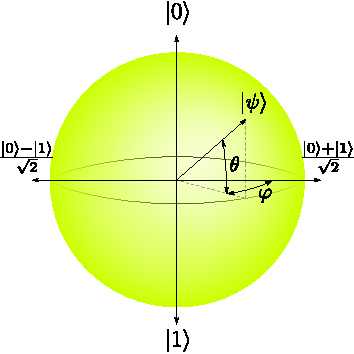
\includegraphics[scale=1]{intro/figs/bloch.pdf}
  \caption{ A quantum state $\ket\psi$ is represented as a point in the surface of the Bloch sphere. The angle theta contains information about the overlap between the state $\ket\psi$ and the basis states $\ket 0$ and $\ket 1$, whereas the angle $\varphi$ describes a phase. \label{fig1:bloch}}
\end{figure}

We will not go into details about quantum computation and quantum algorithms.
%
This is just an example of the powerful capabilities of a quantum computer, but it is not in the scope of this thesis to convince anyone why we need quantum computers and what can they do for us. A quick Google search will already mention some of its applications in internet security, research, etc.
%
We will instead focus on the most essential part of quantum computers: the qubit. A qubit is a quantum bit. It is the analog of a bit in a classic computer but it is not limited to be either in the state 0 or 1. A qubit can be in any quantum superposition of the states $\ket 0$ and $\ket 1$. Qubits are often represented as points in the surface of a sphere: the Bloch sphere. Indeed, any qubit can be expressed as
\begin{align}
\ket{\psi (\theta,\varphi)}  = {}&{} \cos\frac{\theta}{2}\ket 0 + e^{i\varphi} \sin\frac{\theta}{2}\ket 1,
\end{align}
up to an overall phase,
where $\theta$ and $\varphi$ are the polar and azimuthal angles in the Bloch sphere of Fig.~\ref{fig1:bloch}. The states $\ket 0$ and $\ket 1$ denote the north and south poles, respectively, of the sphere.





A qubit is thus a quantum mechanical two-level system, and we need to find a physical implementation of this two-level system if we want to create a quantum computer. When one thinks about two-level quantum systems the first thing that comes to mind is probably the spin of an electron. That is text-book physics. And that is (maybe) what Daniel Loss and David DiVincenzo thought when they wrote their seminal paper on quantum computation using quantum dots~\cite{Loss1998}.


The idea is very simple: If we can localize one electron and manipulate its spin, we can use the spin states $\ket\ua$ and $\ket \da$ as the qubit states. We also need a mechanism to initialize the qubit into any desired quantum state, read out the output state after running a quantum algorithm and we must also be able to couple this qubit to, at least, another qubit to perform two-qubit gates~\cite{DiVincenzo2000a,Nielsen2010}. In Ref.~\cite{Loss1998} the authors address all these issues and propose to localize the electrons in \textit{quantum dots}.



\section{Quantum dots}

\begin{figure}
  \centering
  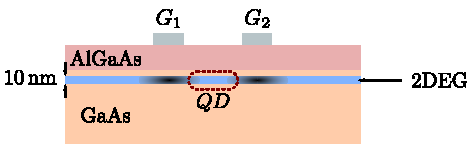
\includegraphics[scale=1]{intro/figs/2deg.pdf}
  \caption{ A 2DEG is formed e.g., close to the interface between a GaAs/AlGaAs heterojunction~\cite{Hanson2007}. It consists of a thin layer ($\sim 10$nm) where electrons can have a high mobility. Top gates ($G_{1}$ and $G_{2}$), lithographically grown, can create a depletion zone in the 2DEG (dark areas), isolating a small region where we can trap one or a few excess electrons (the region enclosed by the dashed red curve). This is a quantum dot.  \label{fig1:2deg}}
\end{figure}

A quantum dot is a potential well that can trap one or a few electrons (or holes). They are typically fabricated in semiconductors, in a two-dimensional electron gas (2DEG). We can think of a 2DEG as a surface in a semiconductor where electrons occupy the conduction band and, thus, can move relatively freely. A 2DEG can be created in Si MOSFETs, in Si/Ge heterostructures, in GaAs/AlGaAs, etc, and in all cases the electrons are confined in a triangular potential along the $z$ direction only, but are unbounded in the $x$-$y$ plane~\cite{Hanson2007,Zwanenburg2013}.


On top of the heterostructure we can put metallic gates. These can be used to apply a localized electric field and create a depletion zone in the 2DEG (see Fig.~\ref{fig1:2deg}). These depletion zones can be engineered to create a whole closed area in the 2DEG where we can trap one or a few electrons. This artificial potential well is a quantum dot.

Once we have a quantum dot we can couple it to a reservoir (by letting electrons tunnel in and out of the quantum dot) and trap one electron. Then we can use the spin of this localized electron for quantum computation.




\section{Making a spin qubit (using quantum dots)}



To understand how a quantum dot-based spin qubit works it is better to see a top view of the device. Fig.~\ref{fig1:2qd} shows a schematic illustration of a system composed of two quantum dots.

\begin{figure}
  \centering
  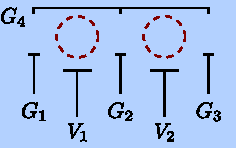
\includegraphics[scale=1]{intro/figs/fig2qd.pdf}
  \caption{ Negative voltages applied to the metallic gates $G_1$, $G_2$, $G_3$ and $G_4$ create a depletion zone in the 2DEG (blue surface). This results in two small isolated islands, the quantum dots, where electrons can be trapped (red circles). The electrochemical potential in the dots can be controlled by the gates $V_1$ and $V_2$. \label{fig1:2qd}}
\end{figure}
The blue surface represents the 2DEG. On top of the device several metallic gates can be individually addressed to create and manipulate the quantum dots: By applying a negative potential on the gates $G_i$, the resulting electric field creates a depletion zone on the 2DEG where electrons are not allowed and a small island where the electrons can be trapped. In Fig.~\ref{fig1:2qd} we show two of such islands, indicated by red dashed circles. These are the quantum dots. We can control the coupling between the two dots by detuning of the gate $G_2$. The gates $G_1$ and $G_3$ can be used to allow electrons in and out of the quantum dots, while the gates $V_1$ and $V_2$ control the electrochemical potential in the dots.

If we now trap one electron in each of the dots we can control its spin with magnetic fields. In fact, with such a simple device, composed of only two quantum dots, it is possible to implement a quantum algorithm~\cite{Watson2018}.

But in this thesis we are not interested in single-spin qubits. The goal of our project is to study decoherence mechanisms in exchange-only spin qubits and mitigate their effects.


